% cassa-photometry -- Workshop Lecture
% Build: pdflatex cassa_photometry_lecture.tex  (run twice for the outline/refs)
% Theme kept to a stock Beamer theme so it compiles anywhere texlive-beamer exists.
\documentclass[10pt,aspectratio=169]{beamer}

\usetheme{Madrid}
\usecolortheme{seahorse}
\setbeamertemplate{navigation symbols}{}
\setbeamertemplate{caption}[numbered]

\usepackage[T1]{fontenc}
\usepackage{lmodern}
\usepackage{amsmath}
\usepackage{booktabs}
\usepackage{listings}
\usepackage{tikz}
\usetikzlibrary{arrows.meta,positioning,shapes.geometric}

\definecolor{cassablue}{RGB}{28,69,135}
\definecolor{cassagrey}{RGB}{240,240,245}
\definecolor{codebg}{RGB}{245,245,248}

\lstset{
  basicstyle=\ttfamily\scriptsize,
  backgroundcolor=\color{codebg},
  breaklines=true,
  columns=fullflexible,
  frame=single,
  framesep=4pt,
  language=Python,
  keepspaces=true,
  showstringspaces=false,
}

% "Aside" frames carry the deeper math; skippable for a lighter audience.
\newcommand{\asidetag}{\hfill{\footnotesize\color{cassablue}[math aside --- optional]}}

\title[cassa-photometry]{The \texttt{cassa-photometry} Pipeline}
\subtitle{From raw pixels to calibrated catalogs, with an error budget the whole way}
\author{CASSA Observatory Workshop}
\date{\today}

\begin{document}

\begin{frame}
  \titlepage
\end{frame}

\begin{frame}{Where we are going}
  \tableofcontents
\end{frame}

% =====================================================================
\section{Motivation \& Overview}
% =====================================================================
\begin{frame}{Why a pipeline?}
  \begin{columns}[T]
    \begin{column}{0.56\textwidth}
      A single night gives you dozens of raw frames. Each one contains, mixed together:
      \begin{itemize}
        \item the astronomical signal you want,
        \item the detector's fingerprint (bias, dark current, flat-field response),
        \item cosmic rays, hot/dead pixels, saturation,
        \item and \textbf{noise} --- which never goes away, only propagates.
      \end{itemize}
      \vspace{0.4em}
      The pipeline turns that pile of raw FITS into \textbf{one calibrated,
      WCS-solved, flux-calibrated catalog} --- and, crucially, tells you the
      \textbf{uncertainty} on every number.
    \end{column}
    \begin{column}{0.44\textwidth}
      \begin{block}{The golden rule}
        A measurement without an error bar is not a measurement.
        \emph{Every stage} of \texttt{cassa-photometry} carries the error forward.
      \end{block}
    \end{column}
  \end{columns}
\end{frame}

\begin{frame}{The four phases}
  \centering
  \scriptsize
  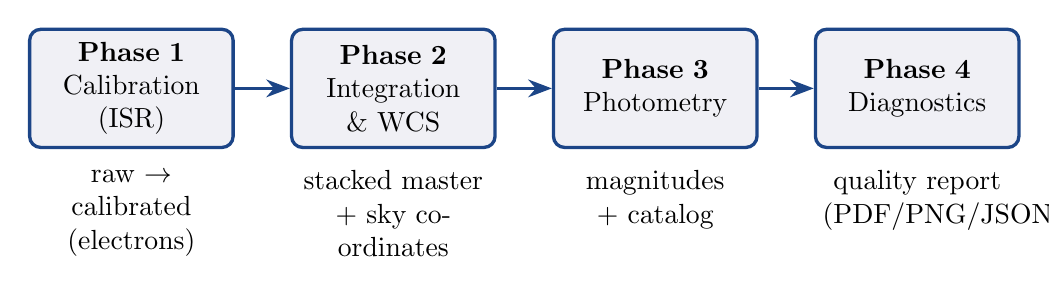
\begin{tikzpicture}[
      node distance=0.55cm and 0.7cm,
      box/.style={rectangle, rounded corners, draw=cassablue, fill=cassagrey,
                  very thick, text width=2.35cm, align=center, minimum height=1.5cm},
      arr/.style={-{Stealth[length=3mm]}, very thick, draw=cassablue}]
    \node[box] (p1) {\textbf{Phase 1}\\ Calibration (ISR)};
    \node[box, right=of p1] (p2) {\textbf{Phase 2}\\ Integration \& WCS};
    \node[box, right=of p2] (p3) {\textbf{Phase 3}\\ Photometry};
    \node[box, right=of p3] (p4) {\textbf{Phase 4}\\ Diagnostics};
    \draw[arr] (p1) -- (p2);
    \draw[arr] (p2) -- (p3);
    \draw[arr] (p3) -- (p4);
    \node[below=0.15cm of p1, text width=2.4cm, align=center] {raw $\rightarrow$ calibrated \\ (electrons)};
    \node[below=0.15cm of p2, text width=2.4cm, align=center] {stacked master \\ + sky coordinates};
    \node[below=0.15cm of p3, text width=2.4cm, align=center] {magnitudes \\ + catalog};
    \node[below=0.15cm of p4, text width=2.4cm, align=center] {quality report \\ (PDF/PNG/JSON)};
  \end{tikzpicture}
  \vspace{1em}
  \begin{itemize}\footnotesize
    \item Each phase is one \texttt{cassa-*} command and one Python sub-package.
    \item They share three things: a config system, logging, and the SCI/ERR/DQ FITS model.
    \item Each writes to its own directory: \texttt{work/phase1} $\rightarrow$ \texttt{phase2} $\rightarrow$ \texttt{phase3} $\rightarrow$ \texttt{phase4}.
  \end{itemize}
\end{frame}

\begin{frame}[fragile]{One command per phase}
\begin{lstlisting}[language=bash]
cassa-calibrate  -i raw/ -o work/phase1    # Phase 1: ISR
cassa-integrate  work/phase1 --yes         # Phase 2: align, stack, WCS
cassa-photometry work/phase2               # Phase 3: zero point + catalog
cassa-diagnose   work/phase2 --raw raw/    # Phase 4: diagnostics

cassa-run -i raw/ -o work/                 # Phases 1->2->3 chained
cassa-verify work/phase3                   # independent sanity check
\end{lstlisting}
  \vspace{0.3em}
  We will meet each of these in the hands-on session. Today: \emph{what each one does and why}.
\end{frame}

% =====================================================================
\section{The Data Model: SCI / ERR / DQ}
% =====================================================================
\begin{frame}{The conceptual spine: three planes, not one}
  Every science image travels as a \textbf{multi-extension FITS} file:
  \vspace{0.5em}
  \begin{center}
  \begin{tabular}{@{}lll@{}}
    \toprule
    Plane & Meaning & Units \\
    \midrule
    \texttt{SCI} (primary) & the science data & electrons ($\rightarrow$ Jy later) \\
    \texttt{ERR} & 1-$\sigma$ per-pixel uncertainty & same as SCI \\
    \texttt{DQ} & integer quality bitmask & --- \\
    \bottomrule
  \end{tabular}
  \end{center}
  \vspace{0.6em}
  \begin{itemize}
    \item \texttt{SCI} in the \emph{primary} HDU $\Rightarrow$ ordinary tools (DS9, \texttt{fits.getdata}, \texttt{solve-field}) still work.
    \item \texttt{ERR} and \texttt{DQ} ride along and are updated by \emph{every} stage.
    \item This is why the final catalog can quote a real \texttt{Mag\_Error}.
  \end{itemize}
\end{frame}

\begin{frame}{The DQ bitmask}
  A pixel can be flagged for several reasons at once --- so we use \textbf{bit flags}
  combined with bitwise OR:
  \vspace{0.5em}
  \begin{center}
  \begin{tabular}{@{}rll@{}}
    \toprule
    Bit value & Name & Set when\dots \\
    \midrule
    0 & \texttt{GOOD} & nothing wrong \\
    1 & \texttt{SATURATED} & pixel $\ge$ saturation ADU \\
    2 & \texttt{BAD\_PIXEL} & hot/dead (from the bad-pixel mask) \\
    4 & \texttt{COSMIC\_RAY} & flagged by LA\,Cosmic \\
    8 & \texttt{NO\_DATA} & NaN / outside the warp footprint \\
    \bottomrule
  \end{tabular}
  \end{center}
  \vspace{0.6em}
  Example: \texttt{DQ = 5 = 1 | 4} $\Rightarrow$ the pixel is both saturated \emph{and} a cosmic ray.
  Downstream, each catalog source inherits the OR of the flags inside its footprint.
\end{frame}

% =====================================================================
\section{Phase 1: Calibration (ISR)}
% =====================================================================
\begin{frame}{Phase 1 --- Instrument Signature Removal}
  Goal: remove the detector's fingerprint and \emph{start} the error budget.
  \begin{enumerate}
    \item Build master \textbf{bias}, \textbf{dark}, \textbf{flat} (median-combined, each with its own uncertainty).
    \item Build a \textbf{bad-pixel mask} from the normalized flat (outliers $<0.5$ or $>1.5$).
    \item For each science frame:
      \begin{itemize}
        \item subtract bias, subtract (scaled) dark, divide by flat;
        \item reject cosmic rays (LA\,Cosmic / \texttt{astroscrappy});
        \item convert ADU $\rightarrow$ electrons via the gain;
        \item assemble the \texttt{DQ} plane (saturation, bad pixel, CR, no-data).
      \end{itemize}
  \end{enumerate}
  \vspace{0.3em}
  \footnotesize Output: \texttt{calibrated\_*.fits} (SCI/ERR/DQ, in electrons). Library: \texttt{ccdproc} does the arithmetic \emph{and} propagates uncertainty automatically.
\end{frame}

\begin{frame}{Phase 1 --- seeding the error budget \asidetag}
  The raw uncertainty of a pixel is Poisson (photon shot noise) plus read noise:
  \[
    \sigma_{\text{ADU}} = \frac{\sqrt{g \cdot \text{ADU} + \text{RN}^2}}{g}
    \quad\text{(electrons after gain: } \sigma_e = \sqrt{g\cdot\text{ADU} + \text{RN}^2}\text{)}
  \]
  where $g$ is the gain (e$^-$/ADU) and RN the read noise (e$^-$).
  \vspace{0.6em}

  Every subsequent operation propagates this in quadrature. Subtracting the master bias:
  \[
    \sigma_{\text{out}} = \sqrt{\sigma_{\text{sci}}^2 + \sigma_{\text{bias}}^2}.
  \]
  Dividing by the flat propagates \emph{relative} errors:
  \[
    \left(\frac{\sigma_{\text{out}}}{\text{sci}_{\text{out}}}\right)^2 =
    \left(\frac{\sigma_{\text{sci}}}{\text{sci}}\right)^2 +
    \left(\frac{\sigma_{\text{flat}}}{\text{flat}}\right)^2 .
  \]
\end{frame}

% =====================================================================
\section{Phase 2: Integration \& Astrometry}
% =====================================================================
\begin{frame}{Phase 2 --- align, stack, solve}
  Goal: combine many calibrated frames into one deep master, and give it sky coordinates.
  \begin{enumerate}
    \item \textbf{Group} frames by object / filter / camera / exposure.
    \item Pick the highest-SNR frame as the \textbf{anchor}.
    \item \textbf{Align} every other frame to the anchor (\texttt{astroalign} matches star patterns; finds shift + rotation + scale).
    \item \textbf{Flux-scale} each frame (median ratio at matched stars), warp the data \emph{and} its variance.
    \item \textbf{Stack} with inverse-variance weighting + outlier rejection.
    \item \textbf{Plate-solve} the stack with Astrometry.net (\texttt{solve-field}) to attach a WCS.
  \end{enumerate}
  \footnotesize Output: \texttt{Master\_*.fits} (SCI/ERR/DQ + WCS) in \texttt{work/phase2}.
\end{frame}

\begin{frame}{Phase 2 --- why inverse-variance weighting? \asidetag}
  If frame $i$ has variance $\text{var}_i$, weight it by $w_i = 1/\text{var}_i$. The stack is
  \[
    \text{master} = \frac{\sum_i w_i\,\text{sci}_i}{\sum_i w_i},
    \qquad
    \text{var}_{\text{master}} = \frac{\sum_i w_i^2\,\text{var}_i}{\left(\sum_i w_i\right)^2}
    = \frac{1}{\sum_i w_i}.
  \]
  \begin{itemize}
    \item Noisy frames contribute less; clean frames dominate. This is the \emph{optimal} linear combination.
    \item Stacking $N$ equal frames shrinks the noise by $\sqrt{N}$ --- the ``depth boost''.
    \item Rejection: sigma-clipping when $\ge 5$ frames, min/max otherwise, kills residual cosmic rays / satellites.
  \end{itemize}
\end{frame}

\begin{frame}[fragile]{Phase 2 --- the astrometry index path (HPC note)}
  \texttt{solve-field} needs multi-GB sky index files. The path is resolved at runtime, in order:
  \begin{enumerate}
    \item \texttt{phase2.astrometry\_index\_dir} in a config YAML, else
    \item the \texttt{CASSA\_ASTROMETRY\_INDEX} environment variable, else
    \item \texttt{./astrometry\_data}.
  \end{enumerate}
\begin{lstlisting}[language=bash]
export CASSA_ASTROMETRY_INDEX=/shared/cassa/astrometry_data
\end{lstlisting}
  \footnotesize On the HPC we keep \emph{one} shared read-only copy and every participant sets the env var.
  (There is no hard-coded path to override --- the pipeline writes a fresh solver config each run.)
\end{frame}

% =====================================================================
\section{Phase 3: Photometry \& Zero Point}
% =====================================================================
\begin{frame}{Phase 3 --- from counts to calibrated magnitudes}
  Goal: put the master stack on a physical scale and catalog every source.
  \begin{enumerate}
    \item \textbf{Detect} stars (\texttt{DAOStarFinder}); measure them with aperture photometry (aperture + sky annulus), using the \texttt{ERR} plane.
    \item \textbf{Cross-match} to a reference catalog; each matched star gives a zero-point estimate.
    \item \textbf{Combine} the per-star zero points $\rightarrow$ one \texttt{MAGZERO} $\pm$ \texttt{MAGZERR} per filter.
    \item \textbf{Flux-calibrate} the image to Janskys; \textbf{catalog} all sources (segmentation + deblending).
  \end{enumerate}
  \footnotesize Output: \texttt{*\_fluxcal.fits} (Jy), \texttt{*\_catalog.csv} (with \texttt{Flux\_Error}, \texttt{Mag\_Error}, \texttt{SNR}, \texttt{FLAGS}), \texttt{*\_segmap.fits}.
\end{frame}

\begin{frame}{Phase 3 --- the zero point, with an error bar \asidetag}
  For each catalog-matched star:
  \[
    m_{\text{inst}} = -2.5\log_{10}(F), \qquad
    \delta m_{\text{inst}} = \frac{2.5}{\ln 10}\,\frac{\delta F}{F} \approx 1.0857\,\frac{\delta F}{F}.
  \]
  \[
    \mathrm{ZP}_i = m_{\text{cat}} - m_{\text{inst}}, \qquad
    \delta \mathrm{ZP}_i = \sqrt{\delta m_{\text{inst}}^2 + \delta m_{\text{cat}}^2}.
  \]
  Combine with sigma-clipping + inverse-variance weighting:
  \[
    \mathrm{ZP} = \frac{\sum_i w_i \mathrm{ZP}_i}{\sum_i w_i}, \quad w_i = 1/\delta\mathrm{ZP}_i^2,
  \]
  and report \texttt{MAGZERR} as the \emph{larger} of the formal error and the scatter's standard error (conservative). Final source magnitude:
  \[
    \delta m = \sqrt{(1.0857\,\delta F/F)^2 + \texttt{MAGZERR}^2}.
  \]
\end{frame}

\begin{frame}{Phase 3 --- the reference catalog}
  The zero point is calibrated \emph{differentially}: detected stars are matched to a
  photometric reference catalog, queried in a filter-aware priority cascade:
  \[
    \textbf{APASS} \;\rightarrow\; \textbf{Pan-STARRS DR2} \;\rightarrow\; \textbf{SDSS DR12}
  \]
  \begin{itemize}
    \item The first catalog to return valid stars for the requested band wins.
    \item Each matched star contributes its catalog magnitude \emph{and} its uncertainty.
    \item These are standardized into one table (\texttt{RAJ2000, DEJ2000, Ref\_Mag, Ref\_Mag\_Err}).
  \end{itemize}
  \footnotesize This step reaches out to the catalog services, so the compute node needs outbound internet.
\end{frame}

% =====================================================================
\section{Phase 4: Diagnostics}
% =====================================================================
\begin{frame}{Phase 4 --- did it actually work?}
  \texttt{cassa-diagnose} inspects each stage and writes a multi-page PDF + PNGs + \texttt{metrics.json}.
  \begin{itemize}
    \item \textbf{Stage 0 (raw):} PSF/FWHM, background, star detection, saturation map.
    \item \textbf{Stage 1 (calibrated):} SCI/ERR/DQ panels, DQ flag counts, the ERR-vs-signal (Poisson) sanity check.
    \item \textbf{Stage 2 (master):} SNR map, depth boost vs a single frame ($\approx\sqrt{N}$), WCS status + plate scale.
    \item \textbf{Stage 3 (photometry):} Mag vs Mag\_Error, SNR vs Mag, number counts / limiting magnitude, star/galaxy split, the recorded ZP + \texttt{MAGZERR}.
  \end{itemize}
  \vspace{0.3em}
  This is where you \emph{read} the error budget you have been carrying the whole way.
\end{frame}

% =====================================================================
\section{Recap \& Hands-on Preview}
% =====================================================================
\begin{frame}{Recap}
  \begin{itemize}
    \item The pipeline is four phases, each a \texttt{cassa-*} command.
    \item The SCI/ERR/DQ model is the spine: uncertainty and quality flags flow from raw pixels to final magnitudes.
    \item Phase 1 seeds the error; Phase 2 stacks it optimally; Phase 3 turns it into calibrated magnitudes with error bars; Phase 4 lets you check it.
    \item Phase 2 plate-solves against a \textbf{local} astrometry index (shared on the HPC, no network); Phase 3's catalog cross-match is a live query.
  \end{itemize}
  \begin{block}{In the hands-on session}
    You will run all four phases on real frames in notebooks \texttt{00}--\texttt{05}, inspecting the SCI/ERR/DQ planes and the catalog at each step.
  \end{block}
\end{frame}

\begin{frame}
  \centering
  \Large Questions?\\[0.5em]
  \normalsize Next: the hands-on notebooks.
\end{frame}

\end{document}
